\chapter{Verification and Validation of Hybrid Method}


This chapter focuses on the verification and the validation of the hybrid method. To perform this feat, we investigated several test-cases: Lamb-Oseen Vortex at $Re=1000$, Clercx-Bruneau Dipole collision at $Re=625$, Impulsively Started Cylinder at $Re=1000$ and the flow around an elliptical airfoil at $Re=5000$.

The verification of \texttt{pHyFlow} was perform as a start where we used the analytical solution of the Lamb-Oseen vortex to verify the velocity and the vorticity field. The Lamb-Oseen vortex problem was also essential for investigating the influences of the solver parameters that impact the accuracy of the coupling. 

The validation of the accuracy of the hybrid solver was performed, once we verified the proper implementation of the hybrid solver. Clercx-Bruneau dipole collision test case was used to investigate the generation of the vorticity in the hybrid scheme and the transfer of this vorticity. This was the first test-cases, where we could confirm the implementation of the vortex panel for the hybrid scheme.


%\section{Comparison of Eulerian vs. Lagrangian solution}
%
%\subsection{Comparison of vorticity contours}
%
%\subsection{Error in maximum vorticity}t
%
%\subsection{Error in $L^2$-norm of velocity}
%
%\subsection{Error in $L^2$-norm of vorticity}

\section{Lamb-Oseen Vortex Evolution}

The Lamb-Oseen Vortex test case simulates the evolution of a laminar vortex core in an unbounded domain. In section \ref{subsec:lagrangianLambOseen}, we used this test case to verify and validate the implementation of the vortex blobs of the Lagrangian solver and in section \ref{subsec:eulerianLambOseen}, we used it to verify the implementation of the Eulerian solver. Therefore, in a similar fashion we will employ this test case to verify the coupling of the hybrid solver. 

The unbounded nature of the problem helps us to neglect the influence of the solid boundary (i.e the wall). Therefore, this test case does not require the panel solver in the Lagrangian solver as we are only concerned with the coupling of the vortex blobs to the Eulerian solver. Thus, we can primarily focus of the vorticity field interpolation error discussed in section \ref{subsubsec:vfie}, and quantitatively present the importance of ensuring conservation of circulation. This is the primary purpose of employing the Lamb-Oseen Vortex test case.

The secondary purpose is to quantify the influences of the discretization on the accuracy of the coupling. A parameter sensitivity analysis was therefore performed to determine their effects on the coupling error. The parameters that determine the spatial discretization of the vortex blobs is nominal particle spacing $h$, and the overlap ratio $Ov$ (see figure \ref{fig:blobOverlap}). The spatial discretization of the Eulerian solver is regarded as a control variable for this test case as its impact was concluded in section \ref{subsec:eulerianLambOseen}. The parameters that determine the temporal discretization of the hybrid method is the time step size of the Eulerian solver $\Delta t_E$ and the time step size of the Lagrangian solver $\Delta t_L$ which are depended according to equation \ref{eq:timeStepDependency} where $k_E$ is the number of Eulerian sub-steps.

The coupling error was quantified my determining the growth of maximum relative error in vorticity $\epsilon$ given by equation \ref{eq:maxRelErrorDef}, approach used in section \ref{subsec:lagrangianLambOseen} and section \ref{subsec:eulerianLambOseen}. 


\subsection{Problem Definition}

The Lamb-Oseen Vortex problem is defined by the vorticity field, equation \ref{eq:lo_voeq}, and the velocity field, equation \ref{eq:lo_veeq}. The hybrid solver is initialized by first assigning the strengths of the vortex blobs using equation \ref{eq:lo_pie}. The Eulerian domain $\Omega_E$ is then initialized using the solution of the Lagrangian solver. Daeninck \cite{Daeninck2006} used this approach to enhance the coupling between the methods ensuring minimum interpolation error.

	\ctable[
		caption = {Summary of the parameters for the Lamb-Oseen vortex evolution. Parameters tabulated below are used for benchmark case.},
		label   = {tab:HLO_pt},
		pos = t,]{lcll}{}{\FL
		
		Parameters 					& Value 	& Unit					& Description \ML
		$\Gamma_c$\T               	& 1 &\si{m^2.s^{-1}} 				& Core strength\\
		$\Omega$               		& $[-0.5,0.5]\times[-0.5,0.5]$ &\si{m}		& Eulerian domain bounds \\
		$\nu$						& $0.001$ &\si{kg.s^{-1}.m^{-1}}& Kinematic viscosity\\
		$ \tau$ 		    		& $100$ 	&\si{s}	& Initial time\\
		$Ov$						& 1 & - & Overlap ratio\\
		$h$							& 0.01 & \si{m} & Nominal blob spacing\\
		$\Gamma_{thres}$			& (\num{1e-14}, \num{1e-14}) & - & Population Control threshold\\
		$h_{grid}$ 					& \numrange{0.007}{0.016} & \si{m} & FE cell diameter span \\
		$ N_{\mathrm{cells}}$ 		& $26448$ 	& -						& Number of mesh cells\\
		$\Delta t_L$				& 0.001 & \si{s} & Lagrangian time step size\\
		$\Delta t_E$				& 0.001 & \si{s} & Eulerian time step size\\		
		$k_E$						& 1 & - & Eulerian sub-steps\\
		$ N_{\mathrm{t-steps}}$ 	& 1000 & -				& Number of time integration steps\\
		$t$ 		    			& \numrange{0}{1} 	&\si{s}			& Simulation time span\\		
		$d_{bdry}$					& $2\cdot{h}$ & \si{m} & Interpolation boundary offset\LL}

	\begin{figure}[h]
	\showthe\columnwidth
	\centering
	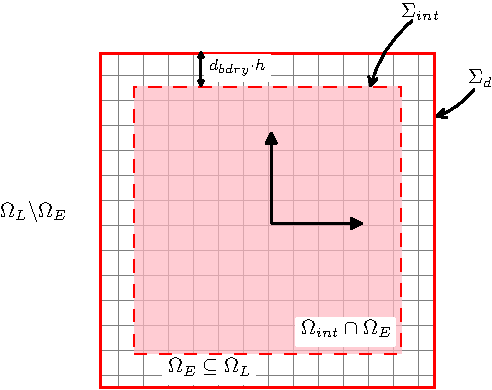
\includegraphics[width=0.5\linewidth]{./figures/hybrid/lambOseen/hlo_dd-crop.pdf}
	\caption{The domain decomposition for the Lamb-Oseen vortex problem, $\Omega_E \subseteq \Omega_L$. The Eulerian domain bounds $\Omega_E = [-1,1]\times[-1,1]$ with Dirichlet boundary $\partial \Omega_{dirichlet}$ [{\color{plotRed}{---}}, solid red] (\emph{not to scale}).}
	\label{fig:HLO_dc}
	\end{figure}

Figure \ref{fig:HLO_dc} shows the Hybrid domain configuration for the Lamb-Oseen Vortex problem with the Lagrangian domain $\Omega_L$ spanning the full fluid domain. The Eulerian domain $\Omega_E$ only resolves the center of the Lamb-Oseen core, $\Omega_E \subseteq \Omega_L$. The domain bounds $[-0.5,-0.5] \times [-0.5,-0.5]$ with a Dirichlet velocity boundary $\Sigma_d$ where the velocity boundary condition is applied as described in section 
\ref{subsec:dbc}. The correction of the Lagrangian domain is performed in the interpolation domain $\Omega_{int}$ according to the procedures described in section \ref{sec:correction}.

The spatial discretization of the Eulerian domain $\Omega_E$ is regarded as the control variable. Therefore, the parameter sensitivity analysis is performed by varying the spatial discretization of the Lagrangian method. The Eulerian domain is discretized with an unstructured mesh formulation using GMSH (see section \ref{subsec:mgugmsh}) having $N_{cells} = 226448$ unstructured cells and grid size $h_{grid}$ spanning $0.007$ to $0.0016$. 

The Lamb-Oseen Vortex problem is defined according to the parameters tabulated in table \ref{tab:HLO_pt}. The core is located at $(0,0)$, where the Eulerian domain $\Omega_E$ is centered. The parameters are chosen such that vorticity $\omega$ and velocity $\mathbf{u}$ is non-zero at the boundary of the Eulerian domain $\Sigma_d$, figure \ref{fig:HLO_dc}. 

The evolution of the Lagrangian solver and the Eulerian solver is performed according to section \ref{sec:evolveLagrangian} and \ref{sec:evolveEulerian} respectively. The Lagrangian solver performs TRS for diffusion of the vortex blobs, see section \ref{subsubsec:srs}. The scheme requires vortex blob redistribution at every step, $f_{redis} = 1$. In conjunction with the redistribution, the population control is performed at every step, $f_{pc}=1$ with $\Gamma_{thre}$ in table \ref{tab:HLO_pt}. 


\subsection{Results and Discussion}

The investigation of the Lamb-Oseen vortex problem is divided into three parts. The first part of the investigation concerns with comparing several stages of the hybrid coupling, section \ref{subsec:UvOvF}, where we compare the uncoupled scheme with the one-way coupled scheme and fully coupled scheme. These successive coupling investigate will help determine the source and quantify the error of the coupling. The second part of the investigation, section \ref{subsubsec:coc} focuses on importance of conservation of circulation that was discussed in section \ref{subsubsec:cc}. The results of the non-conserved and conserved scheme are compared to conclude the importance of conservation of circulation. During these two investigations, the parameters tabulated in table \ref{tab:HLO_pt} are used.

The third and final investigation is dedicated to the parameter sensitivity analysis, section \ref{subsubsec:psa}. Parameters that determine the spatial and temporal discretization of the scheme is investigated to verify the convergence of scheme.

\subsection{Uncoupled vs. One-way Coupled vs. Fully Coupled}
\label{subsec:UvOvF}
To verify the implementation of the hybrid algorithm, we compared several stages of the hybrid coupling with the standard, fully Eulerian test case. The three types of the coupling are as given:

\begin{itemize}
\item \textbf{Uncoupled}: The uncoupled test case involves only Eulerian solver and serves as a benchmark to quantify the error in coupling. The boundary conditions are determined directly from the analytical formulation, equation 	\ref{eq:eLO_veq}.
\item \textbf{One-way coupled}: The one-way coupled test case is a partially coupled hybrid test case where the Eulerian method is evolved using the Lagrangian solution. The correction of the Lagrangian solution is not performed in this scenario. Thus, this case will help us determine the error in evolution Eulerian method using the Lagrangian solution.
\item \textbf{Fully coupled}: The fully coupled test case performs the full coupling strategy described in section \ref{subsec:mcs}. The Eulerian method is evolved using the Lagrangian solution and the Lagrangian solution in the interpolation domain $\Omega_{int}$, figure \ref{fig:HLO_dc} is corrected at the end of each time step. This test case will help us quantify the error in transferring the Eulerian solution to the Lagrangian method.
\end{itemize}
	
	\begin{figure}[h]
     \centering
     \begin{subfigure}[t]{0.45\textwidth}
             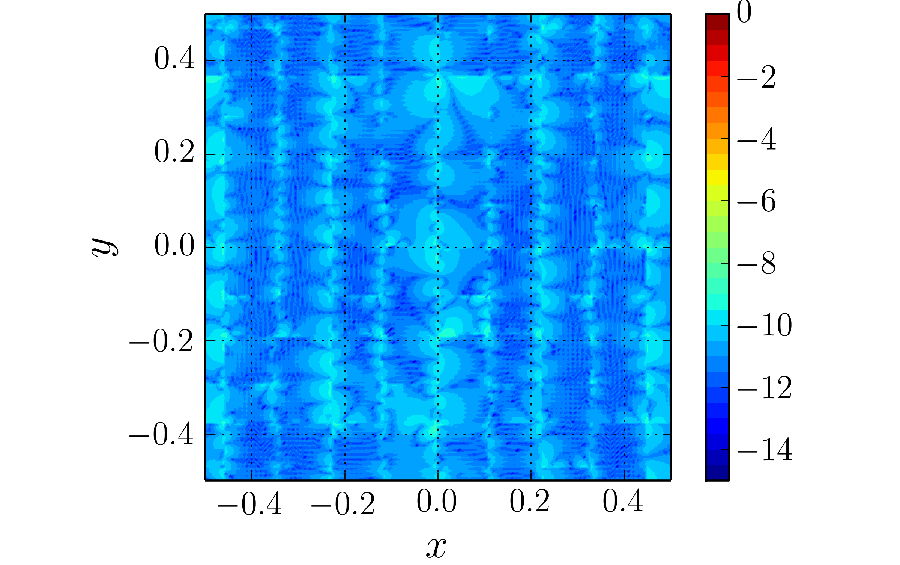
\includegraphics[width=\linewidth]{./figures/hybrid/lambOseen/lambOseen_fully_vErrorInitial_raster.pdf}
             \caption{Velocity}
             \label{fig:lambOseen_oneway_vErrorInitial}
     \end{subfigure}%
     \qquad %add desired spacing between images, e. g. ~, \quad, \qquad etc.
       %(or a blank line to force the subfigure onto a new line)
     \begin{subfigure}[t]{0.45\textwidth}
             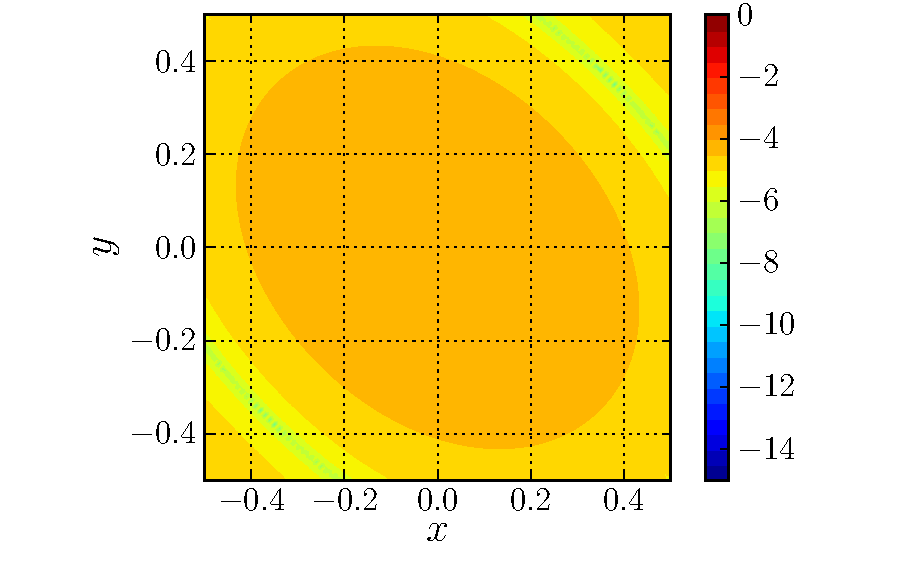
\includegraphics[width=\linewidth]{./figures/hybrid/lambOseen/lambOseen_fully_wErrorInitial_compressed.pdf}
             \caption{Vorticity}
             \label{fig:lambOseen_uncoupled_wErrorInitial}
     \end{subfigure}
     \caption{Initial relative error at $t=0$ inside the Eulerian domain. The figure depicts \textbf{(a)} the relative error in velocity $\mathbf{u}$ and \textbf{(b)} the relative error in vorticity $\omega$.}
     \label{fig:lambOseen_initialError}
	\end{figure}
		
Figure \ref{fig:lambOseen_initialError} depicts the initial relative error in velocity and vorticity inside the Eulerian domain $\Omega_E$. The relative error in velocity is near machine epsilon $\epsilon \le \num{10e-8}$, but the error in vorticity is in the order \num{10e-5}. Similar observation was made in section \ref{subsec:eulerianLambOseen} and arises from the projection error when determining the vorticity from velocity. The error is dependent on the type of discretization and we have second-order velocity space and first-order vorticity space. 

	\begin{figure}[!t]
	\centering
	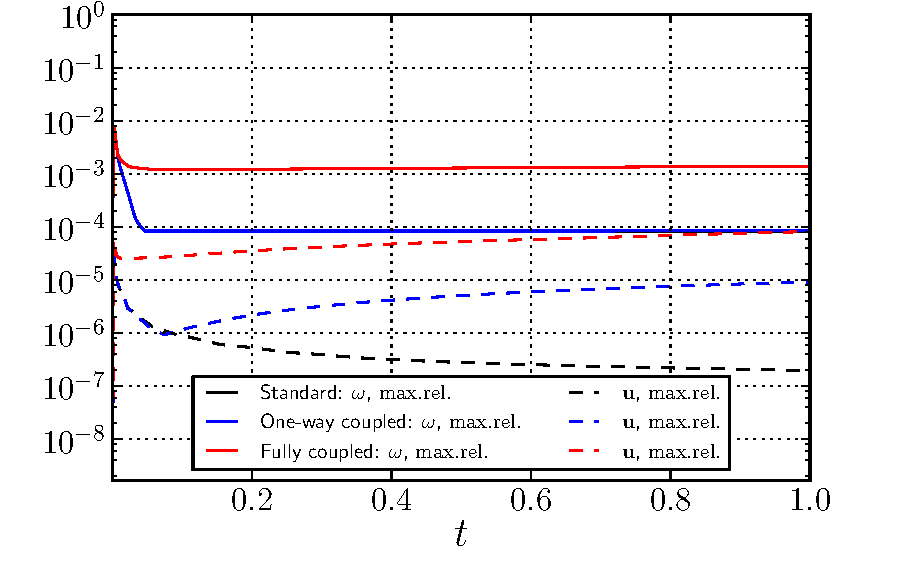
\includegraphics[width=0.6\linewidth]{./figures/hybrid/lambOseen/lambOseen_comparision_compressed.pdf}
	\caption{Comparison of the evolution of the maximum relative error from $t=0$ to $t=1$. The figure compares standard case (\textbf{black}) vs. the one-way coupled case ({\color{plotBlue}{\textbf{blue}}}) vs. the fully coupled case ({\color{plotRed}{\textbf{red}}}). The plot depicts maximum relative error in velocity (dashed), and the maximum relative error in vorticity (solid).}
	\label{fig:lambOseen_comparison}
	\end{figure}

The simulation is evolved from $t=0$ to $t=1$ with $N_{t-steps} = 1000$ Lagrangian and Eulerian time steps using the time step parameters tabulated in table \ref{tab:HLO_pt}. Figure \ref{fig:lambOseen_comparison} shows the evolution of maximum relative error in vorticity $\omega$ and velocity $\mathbf{u}$ of the uncoupled, one-way coupled and the fully coupled cases in the Eulerian domain $\Omega_E$ w.r.t. the analytical solution, equation \ref{eq:lo_voeq}. The initial observation shows the error in velocity is two to three orders of magnitude less than the error in vorticity and occurs due to the projection error. The figure shows that the uncoupled scheme has the lowest error in vorticity and velocity. As the boundary condition is directly obtained from the analytical solution, the error only arises from FE discretization of the Eulerian method. As time progresses, the error in velocity converges around \num{10e-7} and the error in vorticity converges around \num{10e-4}.

The one-way coupled case shows an increase in the velocity field inside the Eulerian domain $\Omega_E$. The increase in error is negligible at the initial stages of the coupling. This states that the discretization error of the analytical solution is well represented using the vortex blobs. At $t=1$, the error in velocity increases by two orders of magnitude from \num{10e-7} to \num{10e-5}. This implies that the error is due to the growth in error of the Lagrangian field. In chapter \ref{ch:lagrangian}, we observed there is an increase in the error due to the circulation processing techniques (population control, remeshing) and the time-marching of the vortex blobs.

The fully coupled case demonstrates that there is further increase in the error in velocity. Moreover, we observe that the there is now an increase in error in vorticity as well. As we are transfer the discrete vorticity field from the Eulerian method to the Lagrangian method it causes an increase in error of the Lagrangian solution. The consequence of this is that now the velocity field resolved by the Lagrangian method has an addition error. The figure depicts this effect, showing an increase in error in velocity. After the first few iteration (around $t=0.2$), there is a measurable difference between the fully coupled and the one-way coupled case. 

	
	\begin{figure}[h]
     \centering
     \begin{subfigure}[t]{0.45\textwidth}
             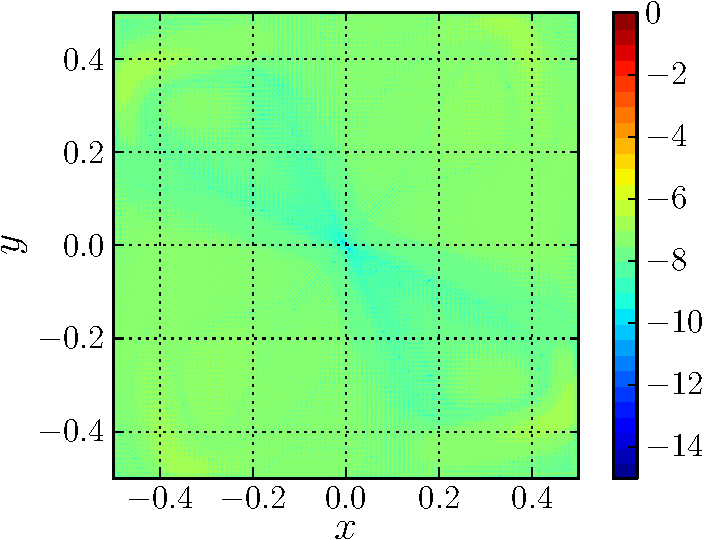
\includegraphics[width=\linewidth]{./figures/hybrid/lambOseent2/lambOseen_uncoupled_vErrorFinal_compressed-crop.pdf}
             \caption{Standard; velocity $\mathbf{u}$}
             \label{fig:lambOseen_uncoupled_vErrorFinal}
     \end{subfigure}%
     \qquad %add desired spacing between images, e. g. ~, \quad, \qquad etc.
       %(or a blank line to force the subfigure onto a new line)
     \begin{subfigure}[t]{0.45\textwidth}
             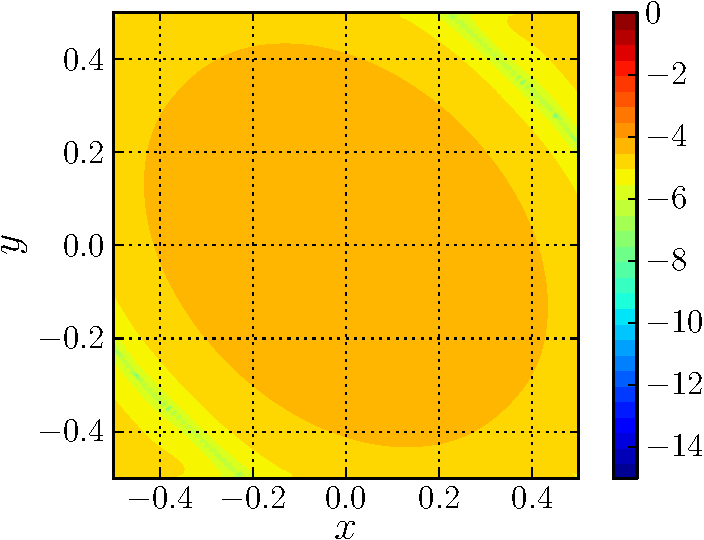
\includegraphics[width=\linewidth]{./figures/hybrid/lambOseent2/lambOseen_uncoupled_wErrorFinal_compressed-crop.pdf}
             \caption{Standard; vorticity $\omega$}
             \label{fig:lambOseen_uncoupled_wErrorFinal}
     \end{subfigure}%       
       
     \begin{subfigure}[t]{0.45\textwidth}
             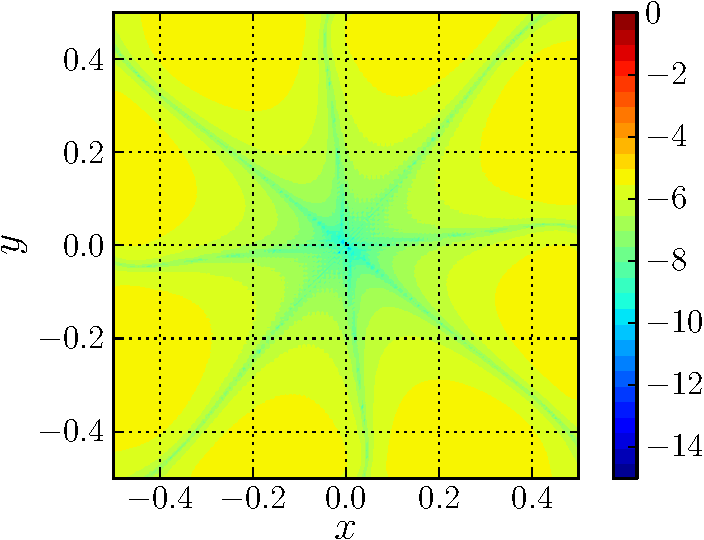
\includegraphics[width=\linewidth]{./figures/hybrid/lambOseent2/lambOseen_oneway_vErrorFinal_compressed-crop.pdf}
             \caption{One-way coupled; velocity $\mathbf{u}$}
             \label{fig:lambOseen_oneway_vErrorFinal}
     \end{subfigure}
     \qquad
     \begin{subfigure}[t]{0.45\textwidth}
             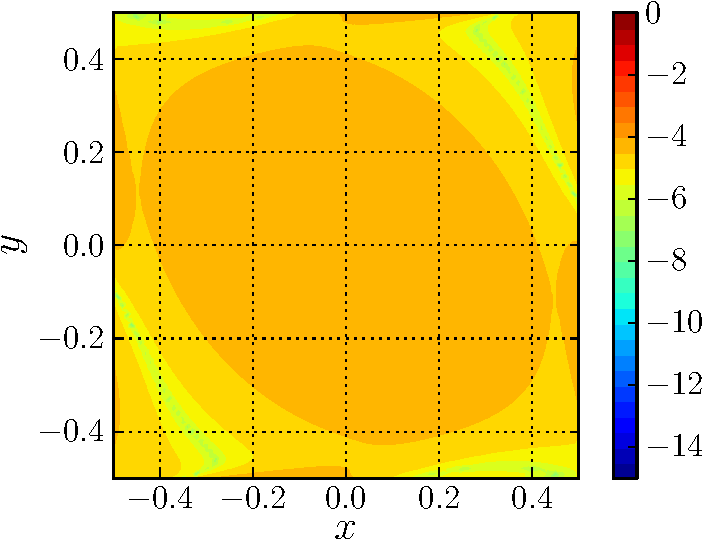
\includegraphics[width=\linewidth]{./figures/hybrid/lambOseent2/lambOseen_oneway_wErrorFinal_compressed-crop.pdf}
             \caption{One-way coupled; vorticity $\omega$}
             \label{fig:lambOseen_oneway_wErrorFinal}
     \end{subfigure}     
   
     \begin{subfigure}[t]{0.45\textwidth}
             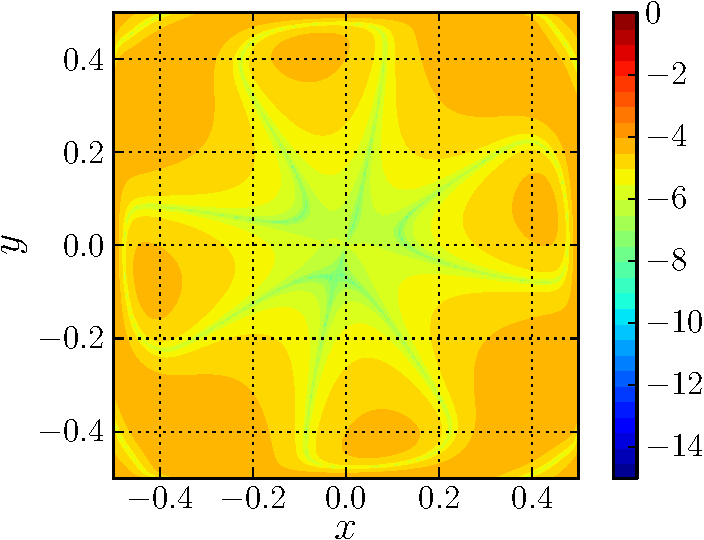
\includegraphics[width=\linewidth]{./figures/hybrid/lambOseent2/lambOseen_fully_vErrorFinal_compressed-crop.pdf}
             \caption{Fully coupled; velocity $\mathbf{u}$}
             \label{fig:lambOseen_fully_vErrorFinal}
     \end{subfigure}     
     \qquad
     \begin{subfigure}[t]{0.45\textwidth}
             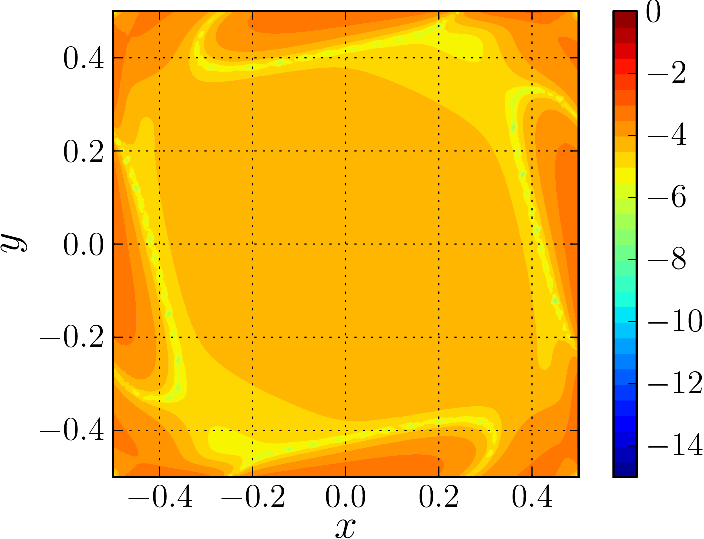
\includegraphics[width=\linewidth]{./figures/hybrid/lambOseent2/lambOseen_fully_wErrorFinal_compressed-crop.pdf}
             \caption{Fully coupled; vorticity $\omega$}
             \label{fig:lambOseen_fully_wErrorFinal}
     \end{subfigure}        
     
     \caption{Initial relative error at $t=0$ inside the Eulerian domain. The figure depicts \textbf{(a)} the relative error in velocity $\mathbf{u}$ and \textbf{(b)} the relative error in vorticity $\omega$.}
     \label{fig:lambOseen_finalError}
	\end{figure}	


\subsubsection*{Conservation of circulation}
\label{subsubsec:coc}

	\begin{figure}[h]
     \centering
     \begin{subfigure}[t]{0.45\textwidth}
             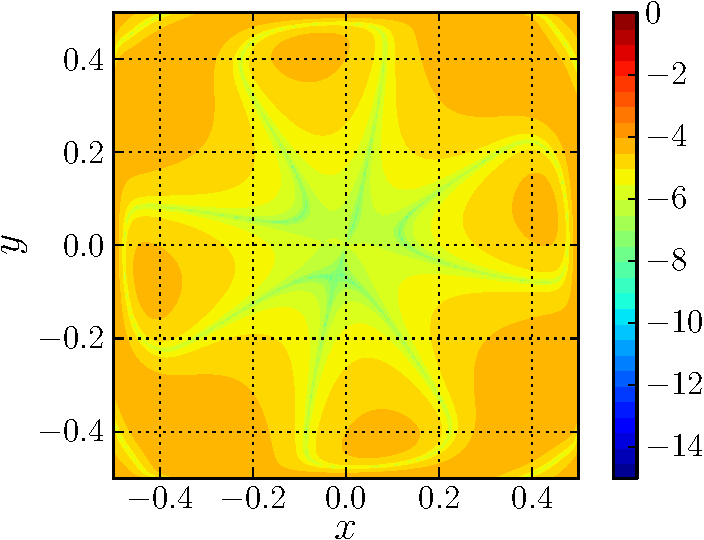
\includegraphics[width=\linewidth]{./figures/hybrid/lambOseent2/lambOseen_fully_vErrorFinal_compressed-crop.pdf}
             \caption{Conservation \texttt{on}; velocity $\mathbf{u}$}
             \label{fig:lambOseen_fullyCon_vErrorFinal}
     \end{subfigure}%
     \qquad %add desired spacing between images, e. g. ~, \quad, \qquad etc.
       %(or a blank line to force the subfigure onto a new line)
     \begin{subfigure}[t]{0.45\textwidth}
             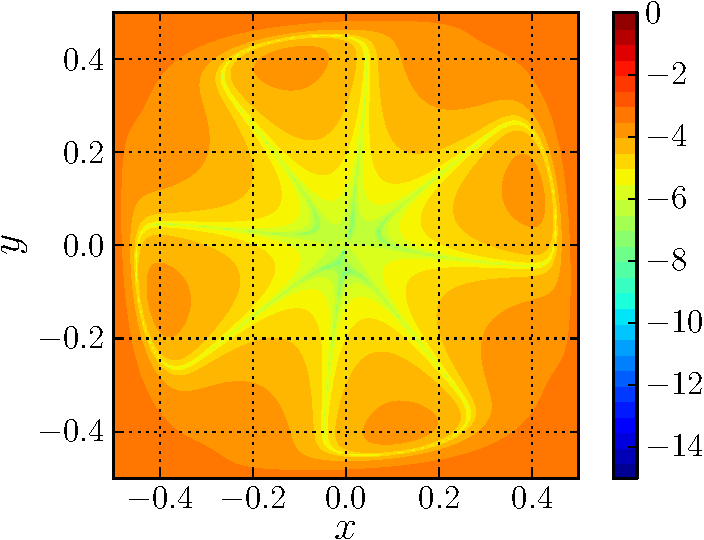
\includegraphics[width=\linewidth]{./figures/hybrid/lambOseent2/lambOseen_fullyCoff_vErrorFinal_compressed-crop.pdf}
             \caption{Conservation \texttt{off}; velocity $\mathbf{u}$}
             \label{fig:lambOseen_fullyCoff_vErrorFinal}
     \end{subfigure}
     
    \begin{subfigure}[t]{0.45\textwidth}
             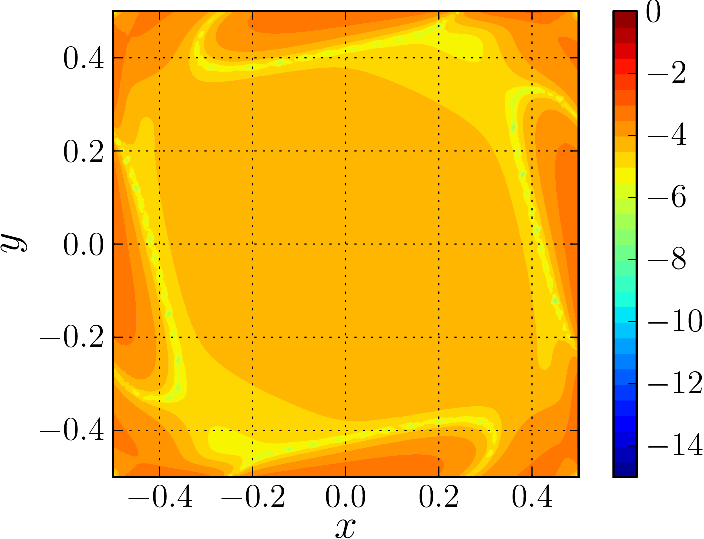
\includegraphics[width=\linewidth]{./figures/hybrid/lambOseent2/lambOseen_fully_wErrorFinal_compressed-crop.pdf}
             \caption{Conservation \texttt{on}; vorticity $\omega$}
             \label{fig:lambOseen_fullyCon_wErrorFinal}
     \end{subfigure}%         
     \qquad     
     \begin{subfigure}[t]{0.45\textwidth}
             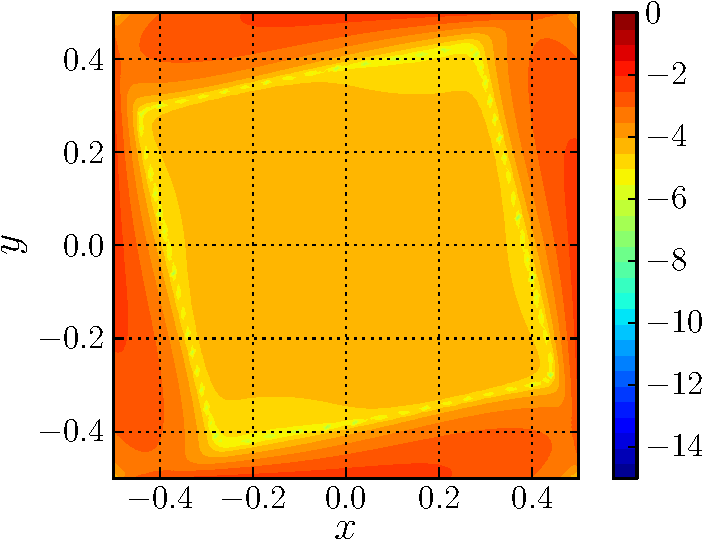
\includegraphics[width=\linewidth]{./figures/hybrid/lambOseent2/lambOseen_fullyCoff_wErrorFinal_compressed-crop.pdf}
             \caption{Conservation \texttt{off}; vorticity $\omega$}
             \label{fig:lambOseen_fullyCoff_wErrorFinal}
     \end{subfigure}  

           
  
     \caption{Initial relative error at $t=0$ inside the Eulerian domain. The figure depicts \textbf{(a)} the relative error in velocity $\mathbf{u}$ and \textbf{(b)} the relative error in vorticity $\omega$.}
     \label{fig:lambOseen_conservation_contourf}
	\end{figure}


	\begin{figure}[h]
     \centering
     \begin{subfigure}[t]{0.45\textwidth}
             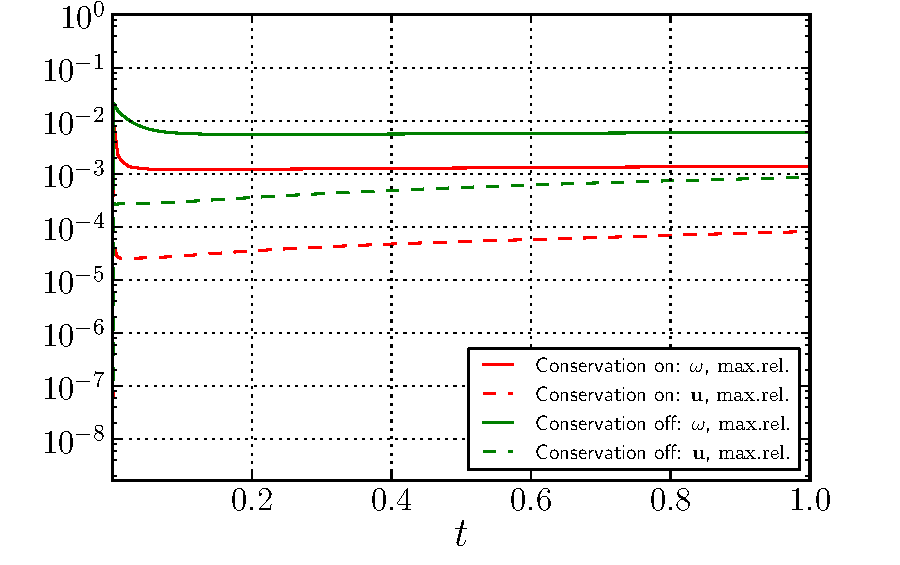
\includegraphics[width=\linewidth]{./figures/hybrid/lambOseent2/lambOseen_comparision_conservation_compressed.pdf}
             \caption{Relative Error in velocity and vorticity}
             \label{fig:lambOseen_comparision_conservation}
     \end{subfigure}%
     \qquad %add desired spacing between images, e. g. ~, \quad, \qquad etc.
       %(or a blank line to force the subfigure onto a new line)
     \begin{subfigure}[t]{0.45\textwidth}
             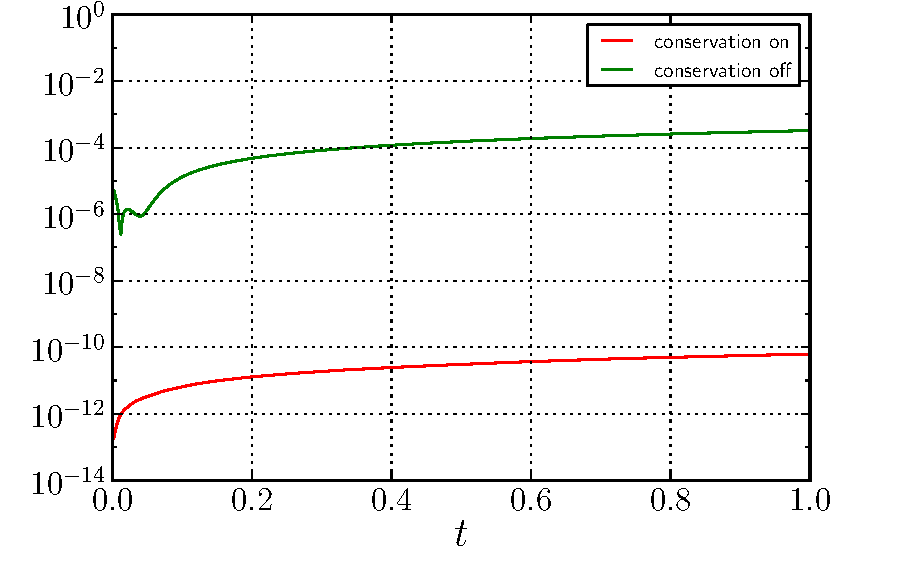
\includegraphics[width=\linewidth]{./figures/hybrid/lambOseent2/lambOseen_comparision_conservation_circulation_compressed.pdf}
             \caption{Error in total circulation $\Gamma$}
             \label{fig:lambOseen_comparision_conservation_circulation}
     \end{subfigure}%       
     \caption{Initial relative error at $t=0$ inside the Eulerian domain. The figure depicts \textbf{(a)} the relative error in velocity $\mathbf{u}$ and \textbf{(b)} the relative error in vorticity $\omega$.}
     \label{fig:lambOseen_conservation_comparisions}
	\end{figure}


\subsubsection{Parameter sensitiviy analysis}
\label{subsubsec:psa}

\subsection{Conclusion}



\section{Clercx-Bruneau Dipole Collision}

\subsection{Problem Definition}

\subsection{Results}

\subsection{Conclusion}

%
%\section{Clercx-Bruneau Dipole Collision}
%
%\subsection{Problem Definition}
%
%\subsection{Results}
%
%\subsection{Conclusion}

%
%	\begin{figure}[h]
%     \centering
%     \begin{subfigure}[t]{0.45\textwidth}
%             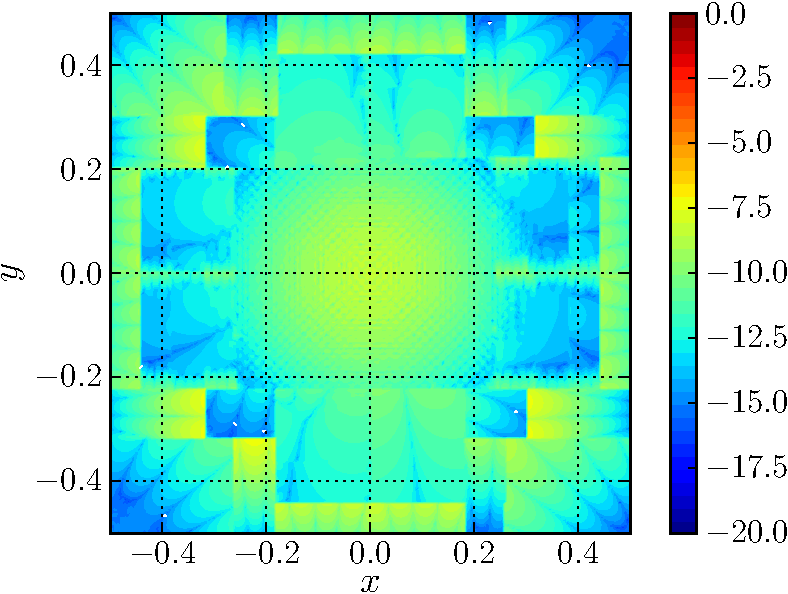
\includegraphics[width=\linewidth]{./figures/hybrid/lambOseen_standard_vErrorInitial_compressed-crop.pdf}
%             \caption{Velocity}
%             \label{fig:lambOseen_standard_vErrorInitial}
%     \end{subfigure}%
%     \qquad %add desired spacing between images, e. g. ~, \quad, \qquad etc.
%       %(or a blank line to force the subfigure onto a new line)
%     \begin{subfigure}[t]{0.45\textwidth}
%             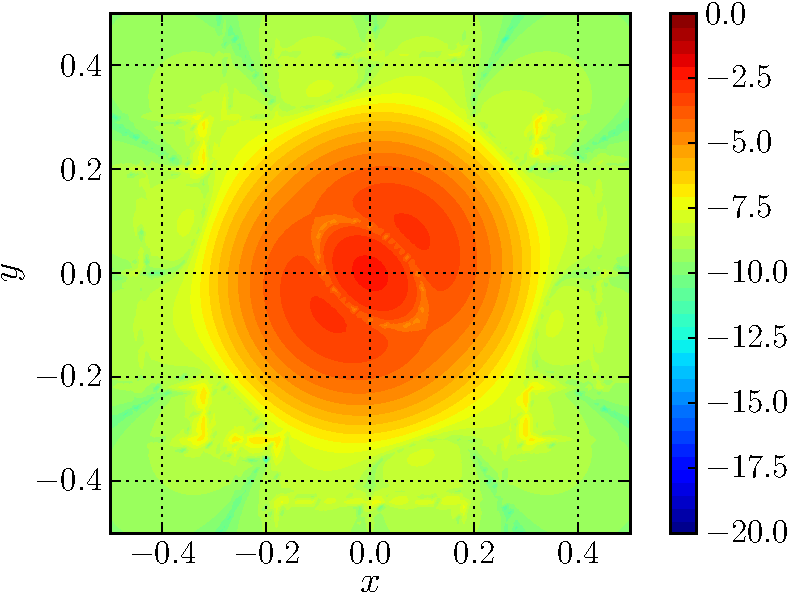
\includegraphics[width=\linewidth]{./figures/hybrid/lambOseen_standard_wErrorInitial_compressed-crop.pdf}
%             \caption{Final Error}
%             \label{fig:lambOseen_standard_wErrorInitial}
%     \end{subfigure}
%     \caption{Initial Error of the Lamb-Oseen vortex}
%     \label{fig:lambOseen_initialError}
%	\end{figure}
%	
	

%	\begin{figure}[h]
%     \centering
%     \begin{subfigure}[t]{0.45\textwidth}
%             \includegraphics[width=\linewidth]{./figures/hybrid/lambOseen_vErrorInitial_compressed-crop.pdf}
%             \caption{Initial Error}
%             \label{fig:lambOseen_vErrorInitial_compressed-crop}
%     \end{subfigure}%
%     ~ %add desired spacing between images, e. g. ~, \quad, \qquad etc.
%       %(or a blank line to force the subfigure onto a new line)
%     \begin{subfigure}[t]{0.45\textwidth}
%             \includegraphics[width=\linewidth]{./figures/hybrid/lambOseen_vErrorFinal_k1_compressed-crop.pdf}
%             \caption{Final Error}
%             \label{fig:lambOseen_vErrorFinal_k1_compressed}
%     \end{subfigure}
%     \caption{Growth in error, velocity max. relative error, dtl=dte, h=0.02, dte=0.001}
%     \label{fig:lambOseen_vError}
%	\end{figure}
%	
%	\begin{figure}[h]
%     \centering
%     \begin{subfigure}[t]{0.45\textwidth}
%             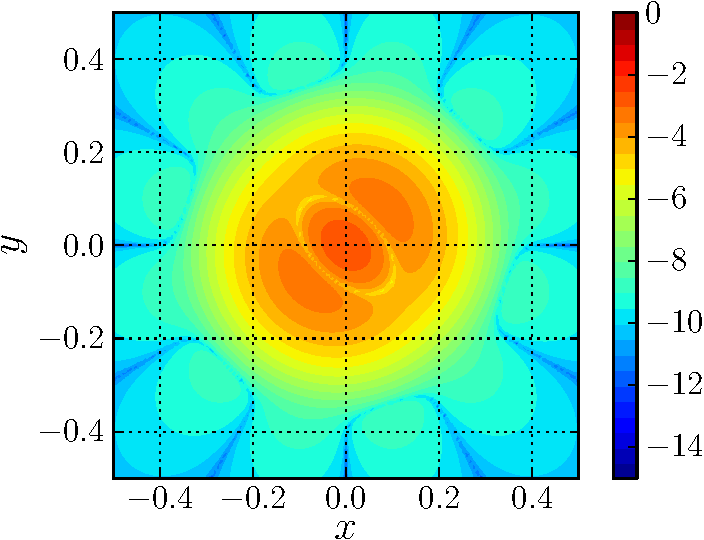
\includegraphics[width=\linewidth]{./figures/hybrid/lambOseen_wErrorInitial_compressed-crop.pdf}
%             \caption{Initial Error}
%             \label{fig:lambOseen_wErrorInitial_compressed}
%     \end{subfigure}%
%     ~ %add desired spacing between images, e. g. ~, \quad, \qquad etc.
%       %(or a blank line to force the subfigure onto a new line)
%     \begin{subfigure}[t]{0.45\textwidth}
%             \includegraphics[width=\linewidth]{./figures/hybrid/lambOseen_wErrorFinal_k1_compressed-crop.pdf}
%             \caption{Final Error}
%             \label{fig:lambOseen_wErrorFinal_k1_compressed}
%     \end{subfigure}
%     \caption{Growth in error, vorticity max. relative error, dtl=dte, h=0.02, dte=0.001}
%     \label{fig:lambOseen_wError}
%	\end{figure}	
	
\subsection{Variation in Lagrangian time step size}	
	
%	\begin{figure}[h]
%		\centering
%		\begin{subfigure}[t]{0.45\textwidth}
%		      \includegraphics[width=\linewidth]{./figures/hybrid/lambOseen_vErrorFinal_k1_compressed-crop.pdf}
%		      \caption{$k=1$}
%		      \label{fig:lambOseen_vErrorFinal_k1}
%		\end{subfigure}%
%		~ %add desired spacing between images, e. g. ~, \quad, \qquad etc.
%		%(or a blank line to force the subfigure onto a new line)
%		\begin{subfigure}[t]{0.45\textwidth}
%		      \includegraphics[width=\linewidth]{./figures/hybrid/lambOseen_vErrorFinal_k2_compressed-crop.pdf}
%		      \caption{$k=2$}
%		      \label{fig:lambOseen_vErrorFinal_k2}
%		\end{subfigure}
%		~
%		\begin{subfigure}[t]{0.45\textwidth}
%		      \includegraphics[width=\linewidth]{./figures/hybrid/lambOseen_vErrorFinal_k5_compressed-crop.pdf}
%		      \caption{$k=5$}
%		      \label{fig:lambOseen_vErrorFinal_k5}
%		\end{subfigure}		
%		~
%		\begin{subfigure}[t]{0.45\textwidth}
%		      \includegraphics[width=\linewidth]{./figures/hybrid/lambOseen_vErrorFinal_k10_compressed-crop.pdf}
%		      \caption{$k=5$}
%		      \label{fig:lambOseen_vErrorFinal_k10}
%		\end{subfigure}			
%		
%		\caption{Variation in the Lagrangian k, velocity max. relative error, dtl=k*dte, h=0.02, dte=0.001}
%		\label{fig:lambOseen_vError_k}
%	\end{figure}
%	
%	
%	\begin{figure}[h]
%		\centering
%		\begin{subfigure}[t]{0.45\textwidth}
%		      \includegraphics[width=\linewidth]{./figures/hybrid/lambOseen_wErrorFinal_k1_compressed-crop.pdf}
%		      \caption{$k=1$}
%		      \label{fig:lambOseen_wErrorFinal_k1}
%		\end{subfigure}%
%		~ %add desired spacing between images, e. g. ~, \quad, \qquad etc.
%		%(or a blank line to force the subfigure onto a new line)
%		\begin{subfigure}[t]{0.45\textwidth}
%		      \includegraphics[width=\linewidth]{./figures/hybrid/lambOseen_wErrorFinal_k2_compressed-crop.pdf}
%		      \caption{$k=2$}
%		      \label{fig:lambOseen_wErrorFinal_k2}
%		\end{subfigure}
%		~
%		\begin{subfigure}[t]{0.45\textwidth}
%		      \includegraphics[width=\linewidth]{./figures/hybrid/lambOseen_wErrorFinal_k5_compressed-crop.pdf}
%		      \caption{$k=5$}
%		      \label{fig:lambOseen_wErrorFinal_k5}
%		\end{subfigure}		
%		~
%		\begin{subfigure}[t]{0.45\textwidth}
%		      \includegraphics[width=\linewidth]{./figures/hybrid/lambOseen_wErrorFinal_k10_compressed-crop.pdf}
%		      \caption{$k=5$}
%		      \label{fig:lambOseen_wErrorFinal_k10}
%		\end{subfigure}			
%		
%		\caption{Variation in the Lagrangian k, velocity max. relative error, dtl=k*dte, h=0.02, dte=0.001}
%		\label{fig:lambOseen_wError_k}
%	\end{figure}		
	
	
%	\begin{figure}[h]
%	\centering
%	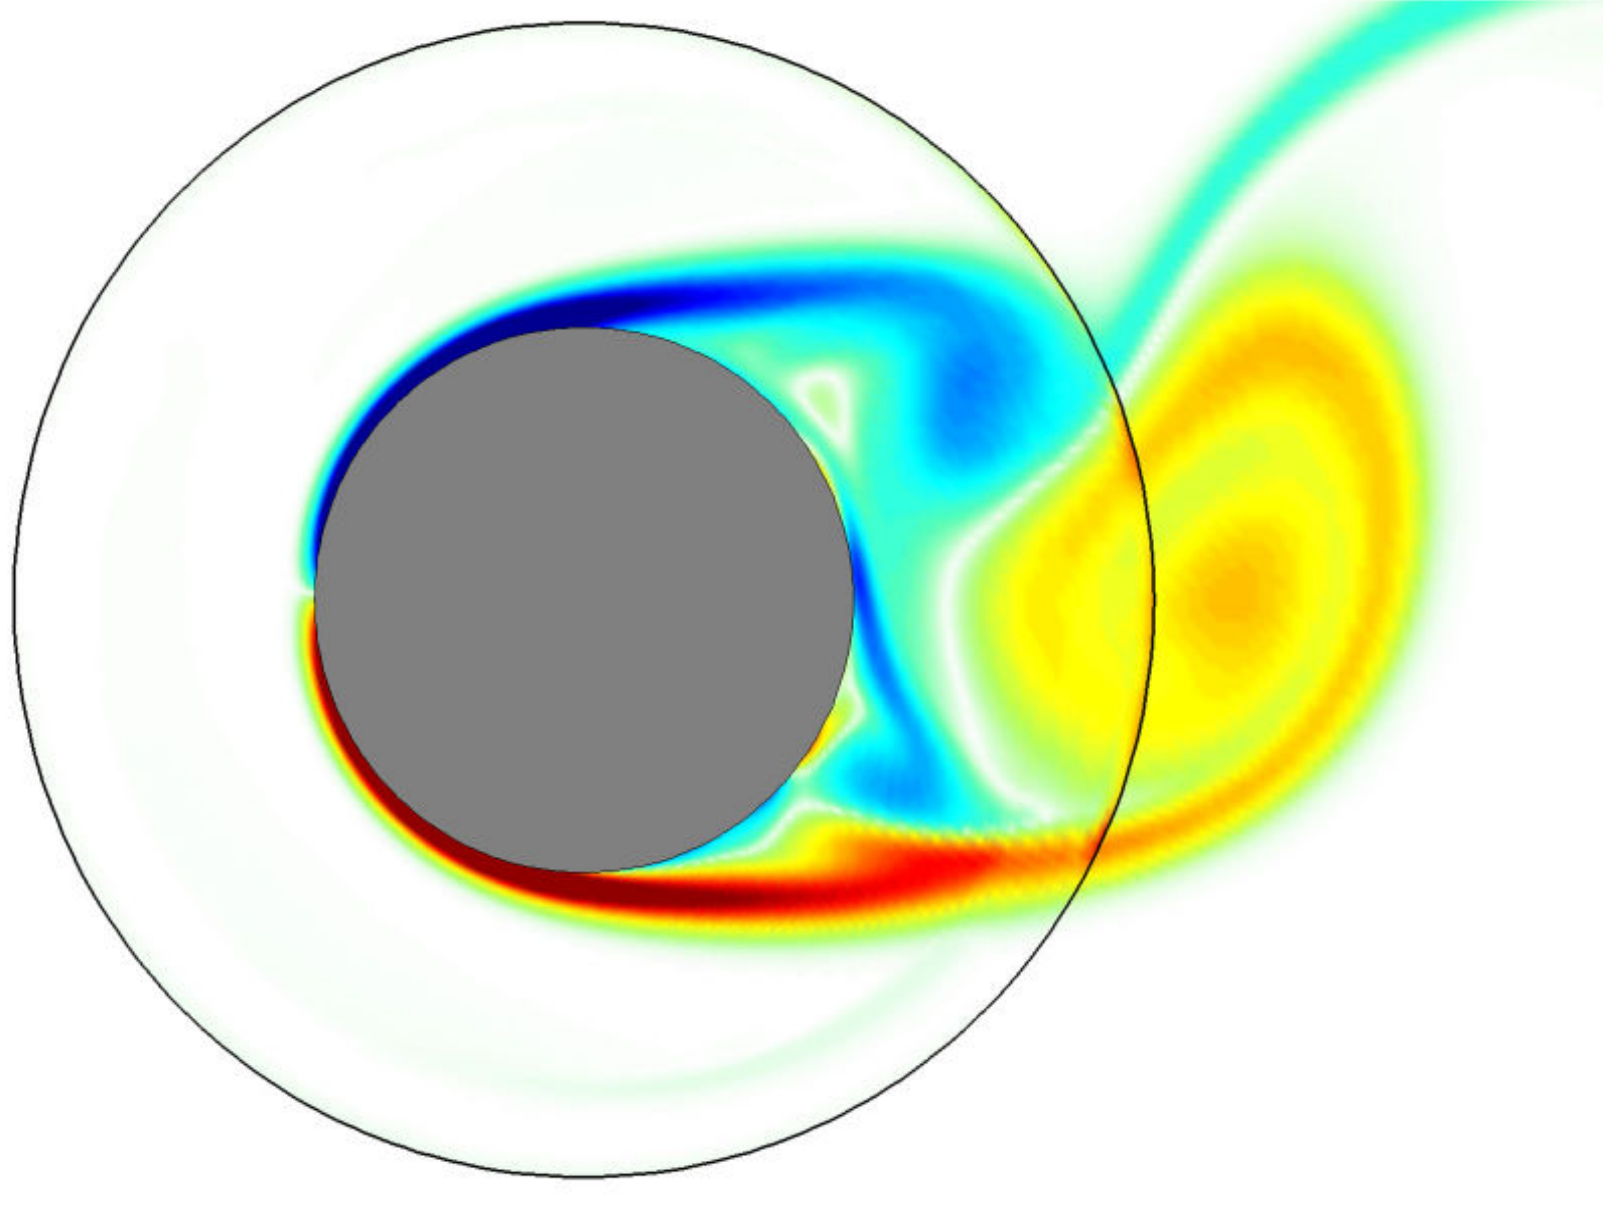
\includegraphics[width=0.5\linewidth]{./figures/hybrid/daeninck_CylinderVorticity.png}
%	\caption{Result of hybrid coupling by Daeninck \cite{Daeninck2006}. The figure shows artificial vorticity at the boundary of the Eulerian domain.}
%	\label{fig:daeninck_CylinderVorticity}
%	\end{figure}




\section{Error in coupling: Verification with Lamb-Oseen vortex}

	\subsection{Generation of artificial vorticity}


\section{Clercx-Bruneau dipole convection at $Re=625$}

	\subsection{Comparison of vorticity contours}
	
	\subsection{Variation in maximum vorticity}
	
	\subsection{Variation in kinetic energy}
	
	\subsection{Variation in enstrophy}

\section{Clercx-Bruneau dipole collision at $Re=625$}

	\subsection{Comparison of vorticity contours}
	
	\subsection{Variation in maximum vorticity}
	
	\subsection{Variation in kinetic energy}
	
	\subsection{Variation in Enstrophy}
	
	\subsection{Variation in Palinstrophy}

\section{Impulsively started cylinder problem at $Re=550$}

	\subsection{Evolution of the wake}
	
	\subsection{Evolution of pressure and friction drag}
	
	\subsection{Evolution of lift}

\section{Moving body}

	\subsection{Error due to pertubation lag}

\section{Proof of concepts}

	\subsection{Multiple cylinder case}
	
	\subsection{Stalled airfoil at $Re=5000$}

\section{Summary}